% =============================================
% File: chapters/methodology.tex
% Chương 3: Phương pháp thực hiện
% =============================================

\chapter{PHƯƠNG PHÁP THỰC HIỆN}
\label{chap:phuongphap}

Chương này trình bày toàn bộ quy trình và phương pháp cụ thể được áp dụng
trong đề tài, gồm hai hướng song song: (1)~\textbf{hướng điều khiển cổ điển}
— thu thập dữ liệu, nhận dạng hàm truyền động cơ, tối ưu tham số bộ điều
khiển tầng bằng giải thuật di truyền, xây dựng mạng ANN dự đoán tham số
thích nghi, và triển khai trên vi điều khiển ESP32; (2)~\textbf{hướng học
tăng cường} — xây dựng môi trường mô phỏng trong Isaac Lab, huấn luyện
chính sách điều khiển bằng thuật toán PPO và xuất trọng số để triển khai
thực tế.


% ==============================================
\section{Quy trình nghiên cứu tổng quan}
% ==============================================

Nghiên cứu được thực hiện theo hai hướng song song với 6 giai đoạn chính:

\begin{enumerate}
    \item \textbf{Giai đoạn 1 — Thu thập dữ liệu thực nghiệm:}
    Vận hành động cơ NF5475 theo giao thức kích thích bậc thang ở 5 mức PWM,
    đọc phản hồi vận tốc qua encoder 200~PPR và ghi log về máy tính qua
    cổng Serial (115\,200~baud).

    \item \textbf{Giai đoạn 2 — Nhận dạng hàm truyền:}
    Sử dụng MATLAB System Identification Toolbox (\texttt{tfest}) để xác định
    hàm truyền $G_{\text{vel}}(s)$ của động cơ; rời rạc hóa bằng phương pháp
    Tustin để phục vụ tối ưu GA.

    \item \textbf{Giai đoạn 3 — Tối ưu bộ điều khiển bằng GA:}
    Áp dụng giải thuật di truyền trên mô hình rời rạc để tìm bộ tham số tối
    ưu $(K_{pp}^*, K_{ip}^*, K_{dp}^*, K_{pv}^*, K_{iv}^*)$ cho bộ điều
    khiển cascade PID-vị trí + PI-vận tốc, tại nhiều mức setpoint.

    \item \textbf{Giai đoạn 4 — Xây dựng và huấn luyện ANN:}
    Từ bộ tham số GA tối ưu tại 9 setpoint vận tốc (250--2250~RPM),
    huấn luyện mạng ANN có khả năng dự đoán tham số PI thích nghi theo
    setpoint và sai số vận tốc hiện tại.

    \item \textbf{Giai đoạn 5 — Triển khai trên ESP32:}
    Cài đặt vòng điều khiển PI với tham số do ANN dự đoán lên vi điều khiển
    ESP32, thực nghiệm vận tốc và đánh giá đáp ứng hệ thống.

    \item \textbf{Giai đoạn 6 — Huấn luyện RL trong Isaac Lab:}
    Song song với hướng điều khiển cổ điển, xây dựng môi trường mô phỏng
    vật lý trong Isaac Lab và huấn luyện chính sách điều khiển chuyển động
    toàn thân bằng thuật toán PPO với curriculum 3 pha dựa trên hiệu suất.
    Sau huấn luyện, trọng số mạng Actor được xuất sang ONNX để triển khai
    thực tế.
\end{enumerate}

% ==============================================
\section{Mô tả hệ thống robot hai chân}
% ==============================================

\subsection{Kiến trúc tổng thể}

Robot Legged V3 là robot hai chân có bánh xe (\textit{wheeled bipedal robot}),
trong đó mỗi chân được dẫn động bởi cơ cấu song song 5-bar. Bánh xe được gắn
tại điểm cuối chân (end-effector), cho phép robot vừa di chuyển bằng bánh vừa
thay đổi chiều cao thân thông qua điều khiển góc khớp.

\begin{figure}[H]
    \centering
    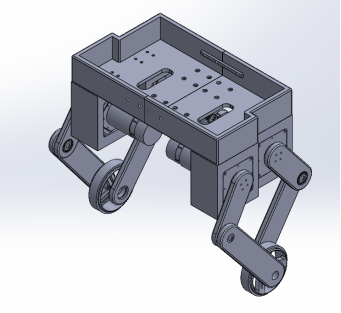
\includegraphics[width=0.45\textwidth]{figure/mohinhtongthe.png}
    \caption{Mô hình tổng thể robot Legged V3}
    \label{fig:robot_overview}
\end{figure}

Robot gồm thân chính phía trên, hai cụm chân đối xứng qua mặt phẳng giữa và
bánh xe đặt tại điểm cuối mỗi chân. Mỗi cụm chân sử dụng hai động cơ NF5475
có encoder để điều khiển hai thanh chủ động; hai thanh bị động tạo thành chuỗi
động học kín, xác định vị trí điểm cuối $P$ để đặt trục bánh xe.

\begin{figure}[H]
    \centering
    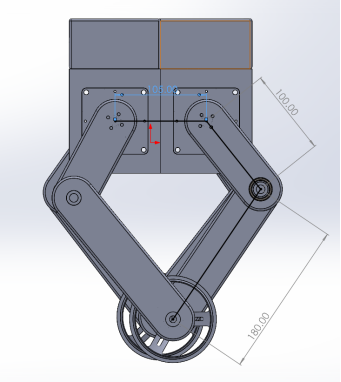
\includegraphics[width=0.45\textwidth]{figure/robotmohinh.png}
    \caption{Mô hình 3D robot Legged V3}
    \label{fig:robot_3d}
\end{figure}

Hệ thống được chia thành ba cấp:
\begin{itemize}
    \item \textbf{Cấp cơ khí:} Khung nhôm định hình, hai cơ cấu 5-bar
    parallel, trục bánh xe.
    \item \textbf{Cấp dẫn động:} Bốn động cơ DC NF5475 (hai mỗi chân)
    kết hợp encoder quang học 200 PPR.
    \item \textbf{Cấp điều khiển:} Vi điều khiển ESP32 WROOM-32, mạch
    driver L298N, giao tiếp Serial/UART với máy tính.
\end{itemize}


\subsection{Cơ cấu 5-bar parallel}

Ký hiệu các thành phần cơ cấu được quy ước trong Bảng~\ref{tab:5bar_notation}.

\begin{table}[H]
    \centering
    \caption{Ký hiệu các thành phần cơ cấu 5-bar parallel}
    \label{tab:5bar_notation}
    \renewcommand{\arraystretch}{1.3}
    \begin{tabular}{|c|l|p{7cm}|}
    \hline
    \textbf{Ký hiệu} & \textbf{Tên} & \textbf{Mô tả} \\
    \hline
    $A_1,\,A_2$ & Khớp chủ động & Hai khớp quay cố định trên thân,
                  truyền động bởi động cơ NF5475 \\
    \hline
    $B_1,\,B_2$ & Khớp bị động & Nối giữa thanh chủ động và thanh bị động \\
    \hline
    $P$         & Điểm cuối     & Vị trí gắn cụm bánh xe \\
    \hline
    $d$         & Khoảng cách gốc & Khoảng cách $A_1A_2$ \\
    \hline
    $L_{act}$   & Thanh chủ động & Chiều dài $A_1B_1$ và $A_2B_2$ \\
    \hline
    $L_{pas}$   & Thanh bị động  & Chiều dài $B_1P$ và $B_2P$ \\
    \hline
    \end{tabular}
\end{table}

Thông số hình học của cơ cấu trong đề tài:

\begin{table}[H]
    \centering
    \caption{Thông số hình học cơ cấu 5-bar parallel}
    \label{tab:5bar_params}
    \renewcommand{\arraystretch}{1.3}
    \begin{tabular}{|l|c|c|}
    \hline
    \textbf{Thông số} & \textbf{Ký hiệu} & \textbf{Giá trị} \\
    \hline
    Khoảng cách hai khớp chủ động & $d = A_1A_2$ & 105 mm \\
    Chiều dài thanh chủ động      & $L_{act}$    & 100 mm \\
    Chiều dài thanh bị động       & $L_{pas}$    & 180 mm \\
    \hline
    \end{tabular}
\end{table}

Ưu điểm so với chân nối tiếp: (i)~độ cứng vững cao hơn do tải phân phối
trên hai thanh bị động, (ii)~khối lượng phần chuyển động nhỏ vì động cơ
đặt tại gốc cố định, (iii)~giảm số bậc tự do cần điều khiển xuống còn 2.


% ==============================================
\section{Thu thập dữ liệu và nhận dạng hàm truyền}
\label{sec:data_sysid}
% ==============================================

\subsection{Quy trình thu thập dữ liệu}

Dữ liệu đặc tính động cơ DC NF5475 được thu thập theo giao thức kích thích
bậc thang (\textit{step-input protocol}). Vi điều khiển ESP32 lần lượt áp
5 mức PWM cố định: $20\%$, $40\%$, $60\%$, $80\%$, $100\%$ (tương ứng 51,
102, 153, 204, 255 đơn vị 8-bit), mỗi mức duy trì trong \textbf{10 giây}.

Vận tốc tức thời được tính sau mỗi chu kỳ lấy mẫu $T_s = 0{,}01\;\text{s}$:
\begin{equation}
    v(k) = \frac{n_{\text{xung}}(k)}{200} \cdot \frac{60}{T_s}
    \qquad [\text{RPM}]
    \label{eq:vel_calc}
\end{equation}
trong đó $n_{\text{xung}}(k)$ là số xung encoder (200~PPR) tích lũy trong
khoảng $[kT_s,\,(k{+}1)T_s)$. Bộ ba $(t,\;v(k),\;u(k))$ được truyền qua
cổng Serial (115\,200~baud) và ghi thành file CSV trên máy tính, thu được 5
file CSV ứng với 5 mức kích thích, tổng khoảng 5\,000 mẫu dữ liệu thô.

\subsection{Tiền xử lý dữ liệu}

\textbf{Chọn file nhận dạng.}
Trong số 5 file thu được, file có mức PWM 80\%
(\texttt{motor\_data\_004.csv}) được chọn làm dữ liệu nhận dạng vì đảm bảo
tỉ số tín hiệu trên nhiễu cao, chưa xảy ra bão hòa tốc độ, và đại diện tốt
cho vùng hoạt động tuyến tính của động cơ.

\textbf{Thêm đoạn trước zero (zero-prepend).}
Để đảm bảo điều kiện ban đầu ổn định cho bộ nhận dạng, $n_x = 100$ mẫu
được ghép vào đầu mỗi chuỗi:
\begin{equation}
    \tilde{u} = [\underbrace{0,\ldots,0}_{n_x},\; u(1),\ldots,u(N)]^{\!\top},
    \qquad
    \tilde{y} = [\underbrace{v(0),\ldots,v(0)}_{n_x},\; v(1),\ldots,v(N)]^{\!\top}
    \label{eq:zero_prepend}
\end{equation}
trong đó chuỗi đầu vào được điền bằng 0 và chuỗi đầu ra được điền bằng
giá trị tốc độ ban đầu $v(0)$.

\textbf{Làm trơn đầu ra.}
Nhiễu đo lường từ encoder được giảm bằng bộ lọc trung bình trượt
(\textit{moving mean}) cửa sổ 5 mẫu:
\begin{equation}
    \hat{y}(k) = \frac{1}{5}\sum_{j=0}^{4} \tilde{y}(k-j)
    \label{eq:smooth}
\end{equation}

\textbf{Chuẩn bị đối tượng nhận dạng.}
Dữ liệu sau xử lý được đóng gói thành đối tượng \texttt{iddata}$(\hat{y},\,\tilde{u},\,T_s)$
trong MATLAB, với $T_s = \overline{\Delta t}$ được tính trực tiếp từ file gốc
(\texttt{Ts = mean(diff(t\_raw))}).

\subsection{Nhận dạng và lựa chọn mô hình tốt nhất}

Hàm \texttt{tfest(data, $n_p$, $n_z$)} được thực thi với toàn bộ tổ hợp:
$n_p \in \{1,2,3,4\}$ cực và $n_z \in \{0,1,\ldots,n_p{-}1\}$ không.
Với mỗi tổ hợp, MATLAB tự động tối ưu hàm truyền liên tục dạng:
\begin{equation}
    G(s) = \frac{b_{n_z}s^{n_z} + \cdots + b_1 s + b_0}
                {s^{n_p} + a_{n_p-1}s^{n_p-1} + \cdots + a_1 s + a_0}
    \label{eq:Gs_form}
\end{equation}
theo phương pháp \textit{prediction error minimization} (PEM). Mô hình được
chọn tự động theo tiêu chí \textbf{FitPercent} cao nhất:
\begin{equation}
    \text{Fit\%} =
    \left(1 - \frac{\lVert y - \hat{y}\,\rVert_2}
                   {\lVert y - \bar{y}\,\rVert_2}\right) \times 100
    \label{eq:fit_pct}
\end{equation}
trong đó $y$ là chuỗi đầu ra thực nghiệm, $\hat{y}$ là đầu ra mô hình mô
phỏng, $\bar{y}$ là giá trị trung bình của $y$.

\subsection{Rời rạc hóa mô hình}

Sau khi chọn được $G_{\text{vel}}(s)$ tốt nhất, mô hình được rời rạc hóa
bằng phương pháp Tustin (xấp xỉ song tuyến):
\begin{equation}
    s \;\longleftarrow\; \frac{2}{T_s}\cdot\frac{z-1}{z+1}
    \label{eq:tustin}
\end{equation}
thu được hàm truyền rời rạc $G_{\text{vel}}(z)$ dưới dạng hai vector hệ số
$\mathbf{b} = [b_0,\ldots,b_{n_b}]$ và $\mathbf{a} = [a_0,\ldots,a_{n_a}]$:
\begin{equation}
    G_{\text{vel}}(z) = \frac{B(z^{-1})}{A(z^{-1})}
    = \frac{b_0 + b_1 z^{-1} + \cdots + b_{n_b} z^{-n_b}}
           {a_0 + a_1 z^{-1} + \cdots + a_{n_a} z^{-n_a}}
    \label{eq:Gz_form}
\end{equation}
Hai vector $\mathbf{b},\mathbf{a}$ này được sử dụng trực tiếp trong vòng lặp
mô phỏng của bước tối ưu GA (Mục~\ref{sec:ga_optim}).


% ==============================================
\section{Tối ưu tham số bộ điều khiển tầng bằng giải thuật di truyền}
\label{sec:ga_optim}
% ==============================================

\subsection{Cấu trúc bộ điều khiển cascade}

Để điều khiển vị trí (góc quay tích lũy, đơn vị encoder counts) động cơ,
đề tài áp dụng cấu trúc \textbf{hai tầng} (\textit{cascade/nested control}):

\begin{itemize}
    \item \textbf{Vòng ngoài — PID vị trí:} Nhận sai số vị trí, xuất
    setpoint vận tốc $v_{sp}$.
    \item \textbf{Vòng trong — PI vận tốc:} Nhận sai số vận tốc, xuất
    tín hiệu PWM $u \in [-255,\,255]$.
\end{itemize}

Phương trình vòng ngoài tại bước $k$:
\begin{align}
    e_p(k) &= p_{sp} - p(k)
    \label{eq:pos_err} \\
    I_p(k) &= \operatorname{clamp}\!\bigl(I_p(k{-}1) + e_p(k)\cdot T_s,\;
              -I_{lim},\; I_{lim}\bigr)
    \label{eq:pos_integrator} \\
    v_{sp}(k) &= \operatorname{clamp}\!\left(
                  K_{pp}\,e_p(k) + K_{ip}\,I_p(k)
                  + K_{dp}\,\frac{e_p(k)-e_p(k{-}1)}{T_s},\;
                  -v_{max},\; v_{max}\right)
    \label{eq:outer_pid}
\end{align}
với $I_{lim} = 1000$ (giới hạn tích phân anti-windup ngoài) và
$v_{max} = 5000$ (clamp setpoint vận tốc).

Phương trình vòng trong với \textbf{anti-windup back-calculation}:
\begin{align}
    e_v(k)      &= v_{sp}(k) - v(k)
    \label{eq:vel_err} \\
    I_v(k)      &= I_v(k{-}1) + e_v(k)\cdot T_s
    \label{eq:vel_int} \\
    u_{raw}(k)  &= K_{pv}\,e_v(k) + K_{iv}\,I_v(k)
    \label{eq:inner_pi} \\
    u(k)        &= \operatorname{clamp}\!\bigl(u_{raw}(k),\; -255,\; 255\bigr)
    \label{eq:pwm_sat}
\end{align}
Khi xảy ra bão hòa ($u_{raw} \neq u$), tích phân vòng trong được hiệu chỉnh
ngược để tránh tích lũy sai số:
\begin{equation}
    I_v(k) \;\leftarrow\; I_v(k)
            - \frac{u_{raw}(k) - u(k)}{\max(K_{iv},\;10^{-6})}
    \label{eq:anti_windup}
\end{equation}

Đáp ứng vận tốc của mô hình động cơ rời rạc được tính theo phương trình
sai phân:
\begin{equation}
    v(k) = \frac{1}{a_0}\!\left[
             \sum_{j=0}^{n_b-1} b_j\,u(k{-}j)
           - \sum_{j=1}^{n_a-1} a_j\,v(k{-}j)
           \right]
    \label{eq:discrete_plant}
\end{equation}
Vị trí tích lũy được ước tính bằng tích phân Euler:
\begin{equation}
    p(k) = p(k{-}1) + v(k)\cdot T_s
    \label{eq:pos_euler}
\end{equation}

\subsection{Hàm mục tiêu}

Hàm mục tiêu được xây dựng theo dạng \textbf{penalty function}, ưu tiên
thời gian xác lập ngắn và ràng buộc mềm chỉ tiêu chất lượng:
\begin{equation}
    J =
    T_{xl}
    + \underbrace{10^5\,\max\!\bigl(OS - 0{,}10,\;0\bigr)}_{\text{phạt vọt lố > 10\%}}
    + \underbrace{10^5\,\max\!\bigl(|e_{ss}| - 0{,}007,\;0\bigr)}_{\text{phạt sai số xác lập > 0,7\%}}
    + \underbrace{10^{-4}\,\overline{u^2}}_{\text{tiết kiệm năng lượng}}
    \label{eq:ga_objective}
\end{equation}
trong đó các đại lượng được định nghĩa:
\begin{itemize}
    \item $T_{xl}$ — thời gian xác lập: thời điểm sớm nhất mà
    $|p(k) - p_{sp}| \leq 0{,}007\,|p_{sp}|$ duy trì liên tục trong cửa sổ
    \textbf{2 giây}; nếu không đạt trong $T_{sim}$, gán $T_{xl} = \text{NaN}$;
    \item $OS = (p_{max} - p_{sp})/|p_{sp}|$ — độ vọt lố tương đối;
    \item $|e_{ss}| = |p(N) - p_{sp}|/|p_{sp}|$ — sai số xác lập tương đối;
    \item $\overline{u^2} = \frac{1}{N}\sum_{k=1}^{N}u(k)^2$ — năng lượng trung
    bình tín hiệu điều khiển.
\end{itemize}
Nếu $J$ là NaN hoặc số phức (hệ mất ổn định), gán $J = 10^8$.

\subsection{Cấu hình giải thuật di truyền}

\begin{table}[H]
    \centering
    \caption{Cấu hình giải thuật di truyền}
    \label{tab:ga_config}
    \renewcommand{\arraystretch}{1.3}
    \begin{tabular}{|l|l|}
    \hline
    \textbf{Tham số} & \textbf{Giá trị} \\
    \hline
    Số biến tối ưu & 5 \\
    Chromosome & $\mathbf{x} = [K_{pp},\;K_{ip},\;K_{dp},\;K_{pv},\;K_{iv}]$ \\
    Cận dưới & $[0,\;0,\;0,\;0,\;0]$ \\
    Cận trên & $[20,\;1,\;1,\;1,\;5]$ \\
    Quy mô quần thể & 80 cá thể \\
    Số thế hệ tối đa & 80 \\
    Tính toán song song & Có (\texttt{UseParallel = true}) \\
    Số lần chạy độc lập & 20 \\
    Setpoint vị trí $p_{sp}$ & 4000 encoder counts \\
    Thời gian mô phỏng $T_{sim}$ & 6 giây \\
    \hline
    \end{tabular}
\end{table}

Miền tìm kiếm theo từng biến:
\begin{equation}
    K_{pp}\!\in[0,20],\quad K_{ip}\!\in[0,1],\quad K_{dp}\!\in[0,1],
    \quad K_{pv}\!\in[0,1],\quad K_{iv}\!\in[0,5]
    \label{eq:ga_bounds}
\end{equation}

\subsection{Quy trình lựa chọn bộ tham số tối ưu}

Để tránh hội tụ cục bộ của một lần chạy GA, thuật toán được lặp lại
$n_{train} = 20$ lần với hạt ngẫu nhiên khác nhau (\texttt{rng('shuffle')}).
Sau mỗi lần chạy, bộ tham số $\mathbf{x}^*$ được đánh giá lại bằng hàm
\texttt{simulate\_response} để tính chính xác các chỉ số đáp ứng.

Quy trình chọn lọc gồm hai bước:

\begin{enumerate}
    \item \textbf{Lọc điều kiện cứng:} Chỉ chấp nhận ứng viên thỏa đồng thời
    cả ba điều kiện:
    \begin{equation}
        OS \leq 10\%
        \quad\wedge\quad
        |e_{ss}| \leq 0{,}7\%
        \quad\wedge\quad
        T_{xl} < \infty
        \label{eq:hard_constraints}
    \end{equation}

    \item \textbf{Chọn theo tiêu chí phụ:} Trong tập ứng viên hợp lệ
    $\mathcal{C}$, chọn bộ có thời gian xác lập nhỏ nhất:
    \begin{equation}
        \mathbf{x}^*_{\text{final}}
        = \operatorname*{arg\,min}_{\mathbf{x}\in\mathcal{C}}\; T_{xl}(\mathbf{x})
        \label{eq:final_selection}
    \end{equation}
\end{enumerate}

Bộ tham số tối ưu cuối cùng
$(K_{pp}^*,\,K_{ip}^*,\,K_{dp}^*,\,K_{pv}^*,\,K_{iv}^*)$
được lưu thành file CSV tại đường dẫn
\texttt{Data\_Gain/best\_gain\_\{p\_sp\}.csv} kèm các chỉ tiêu
$OS$, $|e_{ss}|$, $T_{xl}$, phục vụ giai đoạn huấn luyện ANN.


% ==============================================
\section{Xây dựng và huấn luyện mạng ANN}
\label{sec:ann_train}
% ==============================================

\subsection{Mục tiêu và dữ liệu huấn luyện}

Mục tiêu của mạng ANN là dự đoán cặp tham số PI vận tốc tối ưu
$(K_{pv},\,K_{iv})$ tương ứng với setpoint vận tốc $v_{req}$ và sai số
vận tốc hiện tại $e_{vel} = v_{req} - v_{cur}$, thay thế cho bảng tra tĩnh
cố định. Điều này cho phép bộ điều khiển thích nghi với điều kiện vận hành
thực tế.

\textbf{Tập dữ liệu huấn luyện} được xây dựng từ kết quả GA ở
Mục~\ref{sec:ga_optim}: tại mỗi trong 9 setpoint vận tốc
$v_{req} \in \{250,\, 500,\, \ldots,\, 2250\}$~RPM (bước 250~RPM),
giải thuật di truyền trả về cặp $(K_{pv}^*,\, K_{iv}^*)$ tối ưu cho
vòng PI vận tốc. Tổng cộng tập huấn luyện gồm $N = 9$ mẫu:
\begin{equation}
    \mathcal{D} = \bigl\{(v_{req}^{(i)},\; e_{vel}^{(i)},\;
                          K_{pv}^{*(i)},\; K_{iv}^{*(i)})\bigr\}_{i=1}^{9}
    \label{eq:ann_dataset}
\end{equation}
trong đó $e_{vel}^{(i)}$ được lấy từ phản hồi mô phỏng tại điểm xác lập
ứng với setpoint $v_{req}^{(i)}$.

\subsection{Kiến trúc mạng}

Mạng ANN được thiết kế với kiến trúc MLP bốn lớp (hai lớp ẩn):

\begin{table}[H]
    \centering
    \caption{Kiến trúc mạng ANN dự đoán tham số PI}
    \label{tab:ann_arch}
    \renewcommand{\arraystretch}{1.3}
    \begin{tabular}{|c|c|c|c|}
    \hline
    \textbf{Lớp} & \textbf{Số nơron} & \textbf{Kích hoạt} & \textbf{Chú thích} \\
    \hline
    Đầu vào   & 2  & —    & $[v_{req},\; e_{vel}]$ \\
    Ẩn 1      & 8  & ReLU & + Dropout $p = 0{,}1$ \\
    Ẩn 2      & 16 & ReLU & + Dropout $p = 0{,}1$ \\
    Đầu ra    & 2  & Tuyến tính & $[K_{pv},\; K_{iv}]$ \\
    \hline
    \end{tabular}
\end{table}

Hàm kích hoạt ReLU được dùng cho các lớp ẩn (xem lý thuyết tại
Mục~\ref{sec:ann_activation}):
\begin{equation}
    \text{ReLU}(x) = \max(0,\, x)
    \label{eq:relu_method}
\end{equation}
Lớp đầu ra tuyến tính (không kích hoạt) để đầu ra có thể nhận giá trị
dương tùy ý, phù hợp với miền giá trị của $(K_{pv}, K_{iv})$.

\subsection{Cấu hình huấn luyện}

\begin{table}[H]
    \centering
    \caption{Siêu tham số huấn luyện mạng ANN}
    \label{tab:ann_train_cfg}
    \renewcommand{\arraystretch}{1.3}
    \begin{tabular}{|l|c|l|}
    \hline
    \textbf{Tham số} & \textbf{Giá trị} & \textbf{Ý nghĩa} \\
    \hline
    Hàm mất mát   & MSE      & $\mathcal{L} = \frac{1}{N}\sum_i\|\hat{y}_i - y_i\|^2$ \\
    Optimizer      & Adam     & Adaptive momentum \\
    Learning rate  & $2\times10^{-3}$ & Tốc độ học \\
    Regularization & L2, $\lambda = 5\times10^{-4}$ & Chống overfitting \\
    Dropout        & $p = 0{,}1$      & Sau mỗi lớp ẩn \\
    Số epoch       & đến hội tụ       & Theo dõi validation loss \\
    \hline
    \end{tabular}
\end{table}

Hàm mất mát tổng hợp (MSE + L2 regularization):
\begin{equation}
    \mathcal{L}_{total} =
    \underbrace{\frac{1}{N}\sum_{i=1}^{N}
        \bigl\|\hat{\mathbf{y}}_i - \mathbf{y}_i\bigr\|^2}_{\text{MSE}}
    + \underbrace{\lambda \sum_{l} \|\mathbf{W}^{(l)}\|_F^2}_{\text{L2 trên trọng số}}
    \label{eq:ann_loss}
\end{equation}
trong đó $\hat{\mathbf{y}}_i = [\hat{K}_{pv}^{(i)}, \hat{K}_{iv}^{(i)}]$
là đầu ra dự đoán, $\mathbf{y}_i = [K_{pv}^{*(i)}, K_{iv}^{*(i)}]$ là
nhãn GA, và $\mathbf{W}^{(l)}$ là ma trận trọng số lớp $l$.

\subsection{Triển khai và tích hợp}

Sau khi huấn luyện, mô hình ANN được lưu và tích hợp vào firmware
ESP32 dưới dạng bảng tra nơron (\textit{look-up neural network}):
tại mỗi chu kỳ điều khiển, ESP32 đưa $(v_{req},\, e_{vel})$ vào mạng,
lấy $(K_{pv}, K_{iv})$ dự đoán rồi đưa trực tiếp vào vòng PI vận tốc
(Mục~\ref{sec:esp32_deploy}). Cơ chế này cho phép tham số PI tự điều
chỉnh liên tục theo điều kiện vận hành mà không cần bảng tra cố định.


% ==============================================
\section{Triển khai bộ điều khiển PI trên ESP32}
\label{sec:esp32_deploy}
% ==============================================

\subsection{Rời rạc hóa và anti-windup}

Bộ điều khiển PI vận tốc được rời rạc hóa bằng phương pháp Euler tiến
với chu kỳ lấy mẫu $\Delta t = 0{,}01\;\text{s}$. Tại mỗi bước $k$:
\begin{align}
    e_{vel}(k) &= v_{req}(k) - v_{cur}(k)
    \label{eq:esp32_err} \\
    I(k) &= \operatorname{clamp}\!\bigl(
             I(k{-}1) + e_{vel}(k)\cdot\Delta t,\;
             -1000,\; +1000\bigr)
    \label{eq:esp32_int} \\
    u(k) &= \operatorname{clamp}\!\bigl(
             K_p\cdot e_{vel}(k) + K_i\cdot I(k),\;
             -255,\; +255\bigr)
    \label{eq:esp32_u}
\end{align}
trong đó $v_{req}(k)$ là setpoint vận tốc (RPM), $v_{cur}(k)$ là vận tốc
đo được từ encoder theo~\eqref{eq:vel_calc}. Giới hạn tích phân
$[\!-1000,\,+1000\!]$ ngăn windup khi tín hiệu điều khiển bão hòa.
Hệ số $K_p,\,K_i$ được tra từ bảng tham số tối ưu thu được ở
Mục~\ref{sec:ga_optim} tương ứng với setpoint vận tốc hiện tại.

\subsection{Vòng điều khiển thời gian thực}

Encoder được đọc qua \textbf{ngắt phần cứng} (\texttt{attachInterrupt},
sườn lên kênh A) để không mất xung ngay cả khi CPU đang xử lý vòng lặp
chính. Vòng lặp chính dùng \texttt{millis()} thay cho \texttt{delay()}
để không chặn ISR (\textit{Interrupt Service Routine}):

\begin{enumerate}
    \item Kiểm tra $\mathit{millis}() - t_{prev} \geq 10\;\text{ms}$.
    \item Đọc bộ đếm xung từ ISR, tính $v_{cur}$ theo~\eqref{eq:vel_calc},
    reset bộ đếm về 0.
    \item Tính sai số $e_{vel}$, cập nhật tích phân $I$, tính $u$.
    \item Ghi $|u|$ ra kênh PWM; ghi chiều quay (IN1/IN2 của L298N) theo
    dấu của $u$.
    \item Xuất log $(t,\,v_{cur},\,u)$ qua Serial (115\,200~baud).
    \item Cập nhật $t_{prev} \leftarrow \mathit{millis}()$.
\end{enumerate}

Cơ chế \texttt{millis()}-based scheduling đảm bảo chu kỳ điều khiển
$\Delta t = 10\;\text{ms}$ ổn định mà không phụ thuộc vào thời gian
thực thi các tác vụ bên trong vòng lặp.


% ==============================================
\section{Huấn luyện chính sách điều khiển bằng Isaac Lab}
\label{sec:isaaclab_train}
% ==============================================

\subsection{Thiết lập môi trường mô phỏng}

Môi trường huấn luyện được xây dựng trên Isaac Lab với lớp nền
\texttt{ManagerBasedRLEnvCfg}. Mặt phẳng mô phỏng (\texttt{terrain\_type = "plane"})
có hệ số ma sát tĩnh $\mu_s = 1{,}5$ và động $\mu_k = 1{,}3$ để phản ánh
điều kiện bề mặt thực tế. Vòng lặp vật lý chạy ở \textbf{200~Hz}
($\Delta t_{sim} = 5\;\text{ms}$); chính sách điều khiển được gọi sau mỗi
\texttt{decimation}~$= 4$ bước vật lý, tức là ở \textbf{50~Hz}
($\Delta t_{ctrl} = 20\;\text{ms}$). Mỗi episode kéo dài tối đa
$T_{ep} = 60\;\text{s}$, tương ứng 3\,000 bước điều khiển.

Tại mỗi lần reset, robot được đặt ngẫu nhiên trong vùng
$(x,y) \in [-5, 5]^2\;\text{m}$, góc yaw $\in [-\pi, \pi]$~rad;
các khớp được nhiễu loạn $\pm 0{,}02$~rad / $\pm 0{,}02$~rad/s để
tăng tính đa dạng trạng thái ban đầu.

\subsection{Không gian hành động}

Chính sách xuất \textbf{8 giá trị hành động} được chia thành hai nhóm:

\begin{table}[H]
    \centering
    \caption{Không gian hành động của robot Legged V3}
    \label{tab:action_space}
    \renewcommand{\arraystretch}{1.3}
    \begin{tabular}{|l|p{5.5cm}|c|l|}
    \hline
    \textbf{Nhóm} & \textbf{Khớp} & \textbf{Số chiều} & \textbf{Chế độ / Tỉ lệ} \\
    \hline
    Khớp hông chủ động
        & \texttt{left\_hip\_joint\_A1}, \texttt{right\_hip\_joint\_A1}
        & 2 & Điều khiển vị trí, scale $= 1{,}0$~rad \\
    Bánh xe
        & \texttt{left\_wheel\_joint}, \texttt{right\_wheel\_joint}
        & 2 & Điều khiển vận tốc, scale $= 5{,}0$~rad/s \\
    \hline
    \multicolumn{2}{|l|}{\textbf{Tổng}} & \textbf{4} & \\
    \hline
    \end{tabular}
\end{table}

Đầu ra thô của mạng neural $a \in [-1, 1]^4$ được nhân với hệ số tỉ lệ
tương ứng trước khi gửi đến bộ điều khiển khớp của Isaac Sim.

\textbf{Lưu ý về cơ cấu 5-bar:} Trong cấu trúc robot hiện tại, chính sách
chỉ điều khiển trực tiếp hai khớp hông A1 (một mỗi chân). Khớp A2 được
cấu hình là \textit{mimic joint} (bám theo A1 qua \texttt{PhysxMimicJointAPI}),
còn các khớp gối B1, B2 là thụ động — bị ràng buộc bởi chuỗi động học kín
của cơ cấu 5-bar được xử lý trong bộ giải vật lý PhysX.

\subsection{Cảm biến mô phỏng}

\subsubsection{IMU ảo trên thân robot}

Isaac Lab đặt một \textbf{IMU ảo} (\texttt{ImuCfg}) tại link gốc
\texttt{base\_link} với chu kỳ cập nhật 10~ms. Cảm biến cung cấp bốn luồng
dữ liệu được đọc trực tiếp từ trạng thái vật lý của PhysX:

\begin{itemize}
    \item \textbf{Gia tốc tuyến tính} $\mathbf{a}_{imu} \in \mathbb{R}^3$ —
    gia tốc tuyến tính của gốc robot trong hệ tọa độ thân, bao gồm thành
    phần trọng lực ($g = 9{,}81\;\text{m/s}^2$ dọc trục $-z$ thế giới).

    \item \textbf{Vận tốc góc} $\boldsymbol{\omega}_{imu} \in \mathbb{R}^3$ —
    vận tốc góc $[\omega_x, \omega_y, \omega_z]^{\top}$ của thân trong hệ
    tọa độ thân.

    \item \textbf{Hướng} $\mathbf{q}_{imu} \in \mathbb{R}^4$ — quaternion
    $[q_w, q_x, q_y, q_z]^{\top}$ biểu diễn góc quay từ hệ thế giới sang
    hệ thân robot.

    \item \textbf{Hướng trọng lực chiếu} $\mathbf{g}_{proj} \in \mathbb{R}^3$ —
    vector trọng lực đơn vị $[0, 0, -1]^{\top}$ (hệ thế giới) được chiếu vào
    hệ tọa độ thân, phản ánh độ nghiêng của robot so với phương đứng.
\end{itemize}

\subsubsection{Cảm biến lực tiếp xúc}

Ba đối tượng \texttt{ContactSensorCfg} theo dõi lực pháp tuyến tại các
vùng tiếp xúc:

\begin{itemize}
    \item \texttt{contact\_forces\_base}: theo dõi tiếp xúc của
    \texttt{base\_link} (điều kiện kết thúc episode nếu lực $> 100$~N).
    \item \texttt{contact\_forces\_right/left}: theo dõi tiếp xúc tại
    các link đùi, ống chân, tấm đệm của từng chân với lịch sử 3 bước
    (\texttt{history\_length}~$= 3$) và bật theo dõi thời gian bay
    (\texttt{track\_air\_time = True}).
\end{itemize}

Ba sensor này được định nghĩa trong scene để phục vụ quan sát và logging;
các điều kiện kết thúc episode dựa trên lực tiếp xúc hiện tại đang tắt
trong quá trình huấn luyện (xem Mục~\ref{sec:terminations}).

\subsection{Không gian quan sát}

Không gian quan sát được chia thành hai nhóm riêng biệt theo kiến trúc
Actor-Critic bất đối xứng (\textit{asymmetric observation}):

\subsubsection{Quan sát của Actor (Policy)}

Actor chỉ sử dụng các tín hiệu khả thi trên phần cứng thực, mô phỏng
đúng những gì cảm biến vật lý cung cấp:

\begin{table}[H]
    \centering
    \caption{Không gian quan sát Actor --- task \texttt{Isaac-Legged-V3-Wheel}}
    \label{tab:obs_policy}
    \renewcommand{\arraystretch}{1.3}
    \begin{tabular}{|l|c|l|}
    \hline
    \textbf{Tín hiệu} & \textbf{Số chiều} & \textbf{Mô tả} \\
    \hline
    \texttt{imu\_lin\_acc}           & 3  & Gia tốc tuyến tính IMU trong hệ thân
                                            $[a_x, a_y, a_z]$ (m/s$^2$) \\
    \texttt{imu\_ang\_vel}           & 3  & Vận tốc góc IMU trong hệ thân
                                            $[\omega_x, \omega_y, \omega_z]$ (rad/s) \\
    \texttt{imu\_orientation}        & 4  & Quaternion hướng thân robot
                                            $[q_w, q_x, q_y, q_z]$ \\
    \texttt{imu\_projected\_gravity} & 3  & Vector trọng lực chiếu trong hệ thân \\
    \texttt{joint\_pos}              & 8  & Góc hiện tại 6 khớp chân + 2 bánh xe (rad) \\
    \texttt{joint\_vel}              & 8  & Vận tốc 6 khớp chân + 2 bánh xe (rad/s) \\
    \texttt{last\_action}            & 8  & Hành động bước trước của chính sách \\
    \texttt{velocity\_cmd}           & 3  & Lệnh vận tốc $[v_x, v_y, \omega_z]$
                                            (m/s, m/s, rad/s) \\
    \texttt{height\_cmd}             & 7  & Lệnh chiều cao thân (vị trí + quaternion
                                            mục tiêu, biến động hiệu quả ở $z$) \\
    \hline
    \textbf{Tổng}                    & \textbf{47} & \\
    \hline
    \end{tabular}
\end{table}

Miền giá trị của các lệnh được lấy mẫu đồng đều tại mỗi lần reset:
$v_x \in [-1{,}0,\,1{,}0]$~m/s, $v_y = 0$~m/s,
$\omega_z \in [-1{,}0,\,1{,}0]$~rad/s,
$z_{target} \in [0{,}25,\,0{,}27]$~m.
Với xác suất 50\% (\texttt{rel\_standing\_envs = 0.5}) lệnh vận tốc được đặt
bằng 0, buộc robot học cả hành vi đứng yên.

\subsubsection{Quan sát của Critic (Value function)}

Critic có thêm quyền truy cập vào trạng thái toàn phần của môi trường —
thông tin không khả dụng trên phần cứng thực nhưng đầy đủ trong mô phỏng:

\begin{table}[H]
    \centering
    \caption{Quan sát bổ sung dành riêng cho Critic}
    \label{tab:obs_critic}
    \renewcommand{\arraystretch}{1.3}
    \begin{tabular}{|l|c|l|}
    \hline
    \textbf{Tín hiệu} & \textbf{Số chiều} & \textbf{Mô tả} \\
    \hline
    \texttt{root\_pos\_w}     & 3  & Vị trí gốc robot trong hệ thế giới (m) \\
    \texttt{root\_quat\_w}    & 4  & Quaternion hướng trong hệ thế giới \\
    \texttt{root\_lin\_vel\_w}& 3  & Vận tốc tuyến tính gốc trong hệ thế giới (m/s) \\
    \texttt{root\_ang\_vel\_w}& 3  & Vận tốc góc gốc trong hệ thế giới (rad/s) \\
    \texttt{base\_lin\_vel}   & 3  & Vận tốc tuyến tính trong hệ thân (m/s) \\
    \texttt{joint\_effort}    & 8  & Mô-men xoắn thực tế 8 khớp (N·m) \\
    \texttt{current\_time}    & 1  & Thời gian hiện tại trong episode (s) \\
    \texttt{remaining\_time}  & 1  & Thời gian còn lại trong episode (s) \\
    \hline
    \multicolumn{2}{|l|}{Tổng bổ sung} & \textbf{26} chiều \\
    \hline
    \multicolumn{2}{|l|}{\textbf{Tổng Critic}} & \textbf{73} chiều (47 + 26) \\
    \hline
    \end{tabular}
\end{table}

Việc cung cấp trạng thái đầy đủ cho Critic giúp ước tính hàm giá trị
$V(s)$ chính xác hơn mà không yêu cầu mạng Actor phải quan sát thông tin
đặc quyền. Sau huấn luyện, chỉ mạng Actor (47 chiều đầu vào) được
xuất sang định dạng ONNX để triển khai trên robot thực.

\subsection{Điều kiện kết thúc episode}
\label{sec:terminations}

Ở giai đoạn huấn luyện hiện tại, chỉ có \textbf{một} điều kiện kết thúc
được kích hoạt:
\begin{itemize}
    \item \textbf{Hết thời gian} (\texttt{time\_out}): episode kết thúc khi
    $t \geq 60\;\text{s}$ (3\,000 bước điều khiển ở 50~Hz).
\end{itemize}
Các điều kiện khác như nghiêng quá giới hạn (\texttt{bad\_orientation}),
vận tốc khớp quá ngưỡng (\texttt{joint\_vel\_limit}) và tiếp xúc bất hợp
lệ (\texttt{illegal\_contact\_*}) hiện được comment out trong config để robot
có đủ thời gian khám phá không gian trạng thái trong giai đoạn đầu huấn
luyện, tránh reset quá sớm làm chậm hội tụ.
Khi episode kết thúc sớm (do bất kỳ điều kiện nào được bật), agent nhận
phần thưởng phạt $r_{term} = -200$.

\subsection{Lệnh điều khiển}

Mỗi episode, Isaac Lab lấy mẫu ngẫu nhiên hai lệnh độc lập và duy trì
chúng trong khoảng thời gian resample trước khi thay bằng lệnh mới:

\begin{table}[H]
    \centering
    \caption{Cấu hình lệnh điều khiển}
    \label{tab:commands_cfg}
    \renewcommand{\arraystretch}{1.3}
    \begin{tabular}{|l|l|l|}
    \hline
    \textbf{Lệnh} & \textbf{Thành phần} & \textbf{Miền giá trị / Cấu hình} \\
    \hline
    \multirow{4}{*}{\texttt{velocity\_command}}
        & $v_x$    & $[-1{,}0,\;+1{,}0]$ m/s \\
        & $v_y$    & $0$ m/s (cố định) \\
        & $\omega_z$ & $[-1{,}0,\;+1{,}0]$ rad/s \\
        & Resample & mỗi $[3,\,5]$ s; 50\% env nhận lệnh 0 (đứng yên) \\
    \hline
    \multirow{2}{*}{\texttt{height\_command}}
        & $z_{target}$ & $[0{,}25,\;0{,}27]$ m (chiều cao thân) \\
        & Resample & mỗi $[3,\,6]$ s; roll/pitch/yaw cố định = 0 \\
    \hline
    \end{tabular}
\end{table}

Tham số \texttt{rel\_standing\_envs = 0.5} đảm bảo một nửa số môi trường
song song luôn nhận lệnh vận tốc bằng 0 trong bất kỳ iteration nào,
giúp chính sách học song song cả kỹ năng di chuyển và giữ thăng bằng khi đứng yên.

\subsection{Sự kiện reset}

Tại mỗi lần khởi động lại episode, hai sự kiện reset được áp dụng:

\begin{itemize}
    \item \textbf{Reset khớp} (\texttt{reset\_joints\_by\_offset}): tất cả
    khớp được đặt về vị trí mặc định cộng nhiễu ngẫu nhiên
    $\Delta q \sim \mathcal{U}(-0{,}02,\,+0{,}02)$~rad,
    vận tốc khớp $\dot{q} \sim \mathcal{U}(-0{,}02,\,+0{,}02)$~rad/s.

    \item \textbf{Reset vị trí thân} (\texttt{reset\_root\_state\_uniform}):
    \begin{align*}
        x,y &\sim \mathcal{U}(-5,\,+5)\;\text{m}, \quad
        \psi \sim \mathcal{U}(-\pi,\,+\pi)\;\text{rad} \\
        \dot{x},\dot{y},\dot{z} &\sim \mathcal{U}(-0{,}02,\,+0{,}02)\;\text{m/s}
    \end{align*}
\end{itemize}

Việc đa dạng hóa trạng thái ban đầu trên diện tích $10\times10\;\text{m}^2$
với góc yaw ngẫu nhiên buộc chính sách học khả năng bám lệnh vận tốc
bất kể hướng xuất phát ban đầu.

\subsection{Hàm phần thưởng}

Tổng phần thưởng tại mỗi bước điều khiển là tổ hợp tuyến tính các số
hạng thuộc ba nhóm: nhiệm vụ chính, ổn định và mượt mà tín hiệu.

\begin{table}[H]
    \centering
    \caption{Tất cả số hạng phần thưởng của task \texttt{Isaac-Legged-V3-Wheel}}
    \label{tab:rewards_full}
    \renewcommand{\arraystretch}{1.3}
    \begin{tabular}{|l|c|p{7.5cm}|}
    \hline
    \textbf{Tên} & \textbf{Trọng số $w$} & \textbf{Ý nghĩa} \\
    \hline
    \multicolumn{3}{|c|}{\textit{Nhiệm vụ chính (task rewards)}} \\
    \hline
    \texttt{termination\_penalty}     & $-200$   & Phạt khi episode kết thúc sớm \\
    \texttt{track\_lin\_vel\_xy\_exp} & $+5{,}0$ & Bám vận tốc tịnh tiến $xy$, $\sigma=0{,}5$ \\
    \texttt{track\_ang\_vel\_z\_exp}  & $+4{,}0$ & Bám vận tốc quay $\omega_z$, $\sigma=0{,}5$ \\
    \texttt{track\_base\_height\_exp} & $+8{,}0$ & Bám chiều cao thân, $\sigma=0{,}15$ \\
    \hline
    \multicolumn{3}{|c|}{\textit{Ổn định (stability)}} \\
    \hline
    \texttt{upright} & $-5{,}0$ & Phạt nghiêng thân RPY $\neq (0,0,0)$ — đọc từ IMU \\
    \hline
    \multicolumn{3}{|c|}{\textit{Mượt mà tín hiệu (smoothness) — áp dụng cho \texttt{.*\_hip\_joint\_A1}}} \\
    \hline
    \texttt{stand\_still}  & $-1{,}5$           & Phạt $L_1$ dao động khớp hông khi $|v_{cmd}|<0{,}2$ \\
    \texttt{joint\_acc}    & $-5\times10^{-5}$  & Phạt gia tốc khớp hông $L_2$ (rung lắc) \\
    \texttt{joint\_torques}& $-1\times10^{-4}$  & Phạt mô-men khớp hông $L_2$ (tiêu thụ điện) \\
    \texttt{action\_rate}  & $-0{,}05$          & Phạt thay đổi hành động đột ngột $L_2$ (toàn bộ 4 chiều) \\
    \hline
    \end{tabular}
\end{table}

Các số hạng tracking sử dụng dạng hàm mũ để tạo gradient không bằng 0
ngay cả khi sai số lớn:
\begin{align}
    r_{v_{xy}} &= w_{v_{xy}} \cdot
        \exp\!\left(-\frac{\|\mathbf{v}_{xy} - \mathbf{v}_{xy}^{cmd}\|^2}{\sigma_{v}^2}\right),
    \quad \sigma_v = 0{,}5
    \label{eq:rew_linvel} \\
    r_{\omega_z} &= w_{\omega_z} \cdot
        \exp\!\left(-\frac{(\omega_z - \omega_z^{cmd})^2}{\sigma_\omega^2}\right),
    \quad \sigma_\omega = 0{,}5
    \label{eq:rew_angvel} \\
    r_{z} &= w_z \cdot
        \exp\!\left(-\frac{(z_{base} - z^{cmd})^2}{\sigma_z^2}\right),
    \quad \sigma_z = 0{,}15
    \label{eq:rew_height}
\end{align}
trong đó $\mathbf{v}_{xy}$ là vận tốc tịnh tiến ngang của thân robot trong
hệ tọa độ yaw-aligned. Các số hạng phạt sử dụng chuẩn $L_1$ hoặc $L_2$, áp dụng lên tập khớp
$\mathcal{J}_{hip} = \{\texttt{left\_hip\_joint\_A1},\,\texttt{right\_hip\_joint\_A1}\}$:
\begin{align}
    r_{still}    &= w_{still} \cdot
        \mathbb{1}[|v_{cmd}| < 0{,}2]\cdot
        \sum_{i \in \mathcal{J}_{hip}} |q_i|
    \label{eq:rew_still} \\
    r_{\ddot{q}} &= w_{acc} \cdot \sum_{i \in \mathcal{J}_{hip}} \ddot{q}_i^2,
    \qquad
    r_{\tau}     = w_{\tau} \cdot \sum_{i \in \mathcal{J}_{hip}} \tau_i^2
    \label{eq:rew_acc_torque} \\
    r_{\Delta a} &= w_{\Delta a} \cdot \sum_{i=1}^{4}(a_k^{(i)} - a_{k-1}^{(i)})^2
    \label{eq:rew_action_rate}
\end{align}

Phần thưởng tổng tại mỗi bước: $R_k = \sum_j r_j^{(k)}$.

\subsection{Thuật toán PPO và cấu trúc mạng}

\subsubsection{Kiến trúc Actor-Critic}

Cả Actor và Critic đều là mạng MLP (\textit{Multi-Layer Perceptron}) 3 lớp
ẩn, dùng hàm kích hoạt ELU, với chuẩn hóa quan sát bằng running mean/std:

\begin{table}[H]
    \centering
    \caption{Kiến trúc mạng Actor-Critic}
    \label{tab:network_arch}
    \renewcommand{\arraystretch}{1.3}
    \begin{tabular}{|l|c|c|c|c|}
    \hline
    \textbf{Mạng} & \textbf{Đầu vào} & \textbf{Lớp ẩn} & \textbf{Đầu ra} & \textbf{Kích hoạt ẩn} \\
    \hline
    Actor  & 47  & $[256 \to 256 \to 256]$ & 8 (tuyến tính) & ELU \\
    Critic & 73  & $[256 \to 256 \to 256]$ & 1 (tuyến tính) & ELU \\
    \hline
    \end{tabular}
\end{table}

Actor xuất phân phối Gaussian với giá trị trung bình $\boldsymbol{\mu}_a$ từ mạng
và độ lệch chuẩn ban đầu $\sigma_{noise} = 0{,}5$ (học được trong quá trình huấn luyện).
Số tham số ước tính:
\begin{itemize}
    \item Actor: $47\times256 + 256\times256 + 256\times256 + 256\times8
                 \approx 145\,\text{K}$ tham số.
    \item Critic: $73\times256 + 256\times256 + 256\times256 + 256\times1
                 \approx 149\,\text{K}$ tham số.
\end{itemize}

\subsubsection{Cấu hình thuật toán PPO}

Thuật toán Proximal Policy Optimization (PPO)~\cite{schulman2017ppo}
được triển khai qua thư viện \texttt{rsl\_rl}. Bảng~\ref{tab:ppo_cfg}
trình bày toàn bộ siêu tham số:

\begin{table}[H]
    \centering
    \caption{Siêu tham số PPO}
    \label{tab:ppo_cfg}
    \renewcommand{\arraystretch}{1.3}
    \begin{tabular}{|l|c|l|}
    \hline
    \textbf{Tham số} & \textbf{Giá trị} & \textbf{Ý nghĩa} \\
    \hline
    \multicolumn{3}{|c|}{\textit{Rollout \& Huấn luyện}} \\
    \hline
    \texttt{num\_steps\_per\_env}    & 24      & Số bước rollout mỗi môi trường / iteration \\
    \texttt{max\_iterations}         & 5\,000  & Tổng số iteration huấn luyện \\
    \texttt{num\_learning\_epochs}   & 5       & Số epoch cập nhật mạng mỗi iteration \\
    \texttt{num\_mini\_batches}      & 4       & Số mini-batch mỗi epoch \\
    \hline
    \multicolumn{3}{|c|}{\textit{PPO Clip \& Loss}} \\
    \hline
    \texttt{clip\_param}             & 0{,}2   & Tham số clip $\epsilon$ của PPO \\
    \texttt{value\_loss\_coef}       & 1{,}0   & Hệ số loss hàm giá trị $c_1$ \\
    \texttt{entropy\_coef}           & 0{,}005 & Hệ số entropy bonus $c_2$ \\
    \texttt{use\_clipped\_value\_loss}& True   & Có clip value loss để ổn định \\
    \hline
    \multicolumn{3}{|c|}{\textit{Optimizer \& Gradient}} \\
    \hline
    \texttt{learning\_rate}          & $10^{-3}$ & Tốc độ học Adam \\
    \texttt{schedule}                & adaptive  & Điều chỉnh lr theo KL divergence thực tế \\
    \texttt{desired\_kl}             & 0{,}01  & Ngưỡng KL mục tiêu để scale learning rate \\
    \texttt{max\_grad\_norm}         & 1{,}0   & Clipping gradient để tránh phát nổ \\
    \hline
    \multicolumn{3}{|c|}{\textit{Ước tính lợi thế (GAE)}} \\
    \hline
    $\gamma$ (\texttt{gamma})        & 0{,}99  & Hệ số chiết khấu phần thưởng tương lai \\
    $\lambda$ (\texttt{lam})         & 0{,}95  & Tham số GAE (trade-off bias/variance) \\
    \hline
    \end{tabular}
\end{table}

Tổng kích thước rollout buffer mỗi iteration với 4\,096 môi trường:
\begin{equation}
    N_{buffer} = N_{envs} \times N_{steps} = 4096 \times 24 = 98\,304\;\text{mẫu}
    \label{eq:buffer_size}
\end{equation}
Kích thước mini-batch: $N_{buffer} / N_{mini} = 98\,304 / 4 = 24\,576$ mẫu.

Ưu thế lợi thế được tính theo GAE (\textit{Generalized Advantage Estimation}):
\begin{equation}
    \hat{A}_t = \sum_{l=0}^{N-1} (\gamma\lambda)^l \delta_{t+l},
    \quad \delta_t = r_t + \gamma V(s_{t+1}) - V(s_t)
    \label{eq:gae}
\end{equation}
Hàm loss tổng hợp:
\begin{equation}
    \mathcal{L}_{PPO} =
    -\underbrace{\mathbb{E}\!\left[\min\!\left(
        \rho_t \hat{A}_t,\;
        \operatorname{clip}(\rho_t, 1{\pm}\epsilon)\hat{A}_t
    \right)\right]}_{\mathcal{L}_{policy}}
    + c_1\,\underbrace{\mathbb{E}\!\left[(V_\theta(s_t) - V_t^{targ})^2\right]}_{\mathcal{L}_{value}}
    - c_2\,\underbrace{\mathbb{E}\!\left[H[\pi_\theta(\cdot|s_t)]\right]}_{\mathcal{L}_{entropy}}
    \label{eq:ppo_loss}
\end{equation}
với $\rho_t = \pi_\theta(a_t|s_t)/\pi_{\theta_{old}}(a_t|s_t)$ là tỉ số
likelihood, $\epsilon = 0{,}2$, $c_1 = 1{,}0$, $c_2 = 0{,}005$.

\subsection{Cấu hình phần cứng và khả năng mở rộng}

\subsubsection{Phần cứng huấn luyện}

\begin{table}[H]
    \centering
    \caption{Thông số GPU huấn luyện --- NVIDIA RTX 3070}
    \label{tab:gpu_spec}
    \renewcommand{\arraystretch}{1.3}
    \begin{tabular}{|l|l|}
    \hline
    \textbf{Thông số} & \textbf{Giá trị} \\
    \hline
    Kiến trúc         & NVIDIA Ampere \\
    CUDA Cores        & 5\,888 \\
    Tensor Cores      & 184 (thế hệ 3) \\
    VRAM              & 8\,GB GDDR6 \\
    Băng thông bộ nhớ & 448\,GB/s \\
    Hiệu năng FP32    & 20{,}3 TFLOPS \\
    Hiệu năng TF32    & $\approx$163 TOPS (với Tensor Cores) \\
    \hline
    \end{tabular}
\end{table}

\subsubsection{Ước tính bộ nhớ GPU khi huấn luyện}

Bộ nhớ GPU được sử dụng bởi ba thành phần chính:
\begin{itemize}
    \item \textbf{Isaac Sim runtime} (PhysX + Omniverse): $\approx 2$--$3$\,GB
    — bao gồm trạng thái khớp/link, collision mesh và dữ liệu vật lý của
    $N_{envs}$ articulation.

    \item \textbf{Rollout buffer}: kích thước mỗi iteration
    \begin{equation*}
        M_{buf} = N_{envs} \times N_{steps} \times (d_{obs,c} + d_{act} + 3)
        \times 4\,\text{byte}
        \approx 4096 \times 24 \times 84 \times 4\;\text{byte}
        \approx 33\;\text{MB}
    \end{equation*}
    ($d_{obs,c} = 73$ chiều Critic + $d_{act} = 8$ + reward/done/value $= 3$).

    \item \textbf{Tham số mạng + optimizer state} (Adam moments):
    $\approx (145 + 149) \times 3 \times 4\;\text{byte} \approx 3{,}5\;\text{MB}$.
\end{itemize}

Tổng ước tính: $\approx 3$--$4$\,GB, phù hợp với 8\,GB VRAM của RTX 3070
khi chạy \textbf{4\,096 môi trường song song}. Nếu tăng lên 8\,192 môi
trường, bộ nhớ PhysX tăng tuyến tính và có thể vượt ngưỡng VRAM,
gây hiện tượng trao đổi bộ nhớ xuống RAM (giảm tốc độ đáng kể).
Cấu hình khuyến nghị cho RTX 3070 là \textbf{2\,048--4\,096 môi trường}.

\subsubsection{Curriculum học dựa trên hiệu suất (Performance-Based)}

Thay vì mở rộng không gian hành động theo số iteration cố định, đề tài
áp dụng chiến lược \textbf{curriculum mở rộng lệnh vận tốc theo hiệu suất
thực tế} của robot. Chiến lược gồm 3 giai đoạn (phase) và chuyển phase khi
robot chứng minh được khả năng làm chủ nhiệm vụ hiện tại, đo bằng
\textbf{Exponential Moving Average (EMA)} của phần thưởng mỗi bước.

\paragraph{Cơ chế EMA.}
Sau mỗi lần reset, phần thưởng tích lũy của các môi trường vừa kết thúc
được chia cho độ dài episode để tính phần thưởng trung bình mỗi bước:
\begin{equation}
    \bar{r}_{term}^{(k)} = \frac{\sum_{t} r_{term}(t)}{T_{ep}}
    \label{eq:per_step_reward}
\end{equation}
EMA được cập nhật với hệ số làm mịn $\alpha_{EMA} = 0{,}03$
(tương đương cửa sổ $\approx 33$ episode):
\begin{equation}
    \hat{r}_{k+1} = (1 - \alpha)\,\hat{r}_k + \alpha\,\bar{r}_{term}^{(k)}
    \label{eq:ema_update}
\end{equation}
Ba luồng EMA được theo dõi độc lập: $\hat{r}_{upright}$, $\hat{r}_{v_{xy}}$,
$\hat{r}_{\omega_z}$.

\paragraph{Điều kiện chuyển phase.}
\begin{itemize}
    \item \textbf{Phase 0 → 1:} Robot phải giữ thân thẳng ổn định:
    \begin{equation}
        \hat{r}_{upright} \;\geq\; (1 - \mathit{MASTERY}) \times w_{upright}
        = 0{,}2 \times (-5{,}0) = -1{,}0
        \label{eq:phase01}
    \end{equation}

    \item \textbf{Phase 1 → 2:} Robot phải bám vận tốc ổn định ở mức thấp:
    \begin{equation}
        \hat{r}_{v_{xy}} \geq \mathit{MASTERY} \times w_{v_{xy}} = 0{,}8 \times 5{,}0 = 4{,}0
        \;\;\text{VÀ}\;\;
        \hat{r}_{\omega_z} \geq \mathit{MASTERY} \times w_{\omega_z} = 0{,}8 \times 4{,}0 = 3{,}2
        \label{eq:phase12}
    \end{equation}
\end{itemize}
với ngưỡng làm chủ $\mathit{MASTERY} = 0{,}80$.

\paragraph{Thay đổi cấu hình theo phase.}
Khi phase chuyển, dải lệnh vận tốc và tỉ lệ môi trường đứng yên
được cập nhật trực tiếp vào \texttt{CurriculumManager}:

\begin{table}[H]
    \centering
    \caption{Cấu hình lệnh vận tốc theo phase curriculum}
    \label{tab:curriculum_phases}
    \renewcommand{\arraystretch}{1.3}
    \begin{tabular}{|c|l|c|c|c|}
    \hline
    \textbf{Phase} & \textbf{Điều kiện chuyển} & $v_x$ (m/s) & $\omega_z$ (rad/s) & \textbf{\% đứng yên} \\
    \hline
    0 & Khởi đầu (mặc định)                        & $[0,\;0]$      & $[0,\;0]$      & 100\% \\
    1 & $\hat{r}_{upright} \geq -1{,}0$           & $[-0{,}5,\;0{,}5]$ & $[-0{,}5,\;0{,}5]$ & 30\% \\
    2 & $\hat{r}_{v_{xy}} \geq 4{,}0$ và $\hat{r}_{\omega_z} \geq 3{,}2$ & $[-1{,}0,\;1{,}0]$ & $[-1{,}0,\;1{,}0]$ & 10\% \\
    \hline
    \end{tabular}
\end{table}

Kiến trúc mạng (đầu vào cố định, 4 chiều hành động) và trọng số không
thay đổi giữa các phase. Chỉ có dải lệnh điều khiển mở rộng dần,
buộc chính sách học từ \textit{đứng thẳng} → \textit{di chuyển chậm}
→ \textit{tốc độ đầy đủ} theo năng lực thực tế của robot.
